\chapter{Literature Review}

\section{Tensegrity Structures}
It is possible to design free-standing structures with axially loaded compression elements in a well crafted network of tensional elements.
Such an arrangement is called a tensegrity structure (tensile integrity). 
Each element of the structure experiences either pure axial compression or pure tension \cite{BuckminsterFuller1975}\cite{Snelson1965}.
The absence of bending or shear forces allows for highly efficient use of materials, 
resulting in lightweight, yet robust systems.

Because the struts are not directly connected, 
tensegrities have the unique property that externally applied forces distribute through the structure via multiple load paths. 
This creates a soft structure, for a soft robot, out of inherently rigid materials.
Since there are no rigid connections within the structure, there are also no lever arms to magnify forces. 
The result is a global level of robustness and tolerance to forces applied from any direction.

%Tensegrity structures are composed of axially loaded compression elements encompassed within a network of tensional elements, and thus each 
%element experiences either pure linear compression or pure tension.  As a result, individual elements can be extremely lightweight as there are no 
%bending or shear forces that must be resisted.  Because the struts are not directly connected, a unique property of tensegrity structures is how externally applied forces distribute through the structure 
%via multiple load paths, creating a system level robustness and tolerance to forces applied from any direction.  
%Because there are no rigid connections within the structure, there are also no lever arms to magnify forces.  Instead, all experienced forces act linearly on each structural element.  Combined with the ability to diffuse forces globally, 
This makes tensegrity robots inherently compliant and extremely well suited for physical interactions with complex and poorly modeled natural environments.  
Active motion in tensegrity robots can be performed by changing cable lengths in parallel, 
enabling the use of many small actuators that work together, rather than individual heavy actuators which work in series.  
There are also many indications that tensegrity properties are prevalent throughout biological systems, 
and the morphology of the SUPERball that we are studying, 
especially when carrying a payload, 
ends up bearing a striking resemblance to the nucleated tensegrity model of cell structure~\cite{Wang2009}\cite{Wang2001}.

\section{Prior Work in Tensegrity Robotics Design}
An important advantage of tensegrity structures with respect to general pin-jointed structures is their increased mass-efficiency due to a high fraction of tensile members.
Tensile members are generally more mass-efficient as they do not need to resist buckling.
A further advantage from a robotics perspective is that forces diffuse in a tensegrity.
There are no lever arms and torques do not accumulate at the joints as in a classic serial manipulator.
Forces distribute through multiple load paths, thus increasing robustness and tolerance to mechanical failure.

%advantages
%applications
The static properties of tensegrities have been thoroughly studied and some basic analysis is discussed in section \ref{modeling}.
On the other hand, few examples are known of truly dynamic motion of these structures.
Early examples of kinematic motion include the work at EPFL's IMAC laboratory~\cite{Fest2004}.
Skelton and Sultan introduced algorithms for the positioning of tensegrity based telescopes and the dynamic control of a tensegrity flight simulator platform~\cite{sultan2000tensegrity}.
Although there were some early efforts at MIT's CSAIL lab, it wasn't until the work of Paul and Lipson at Cornell University that the concept of tensegrity robotics became widespread~\cite{Paul2006a}.
Paul and Lipson were the first to study the properties of dynamic tensegrity structures in hardware and simulation.
A few years later Fivat and Lipson designed the IcoTens, a small actuated tensegrity icosahedron robot, but did not publish results.
In recent years, the BIER lab at the University of Virginia has been studying Central Pattern Generator based control for tensegrity based fish tails,
which is closely related to the control architectures proposed for SUPERball~\cite{Caluwaerts2013rsif,Bliss2012}.
Mirats-Tur has presented design and controls work on various other tensegrity morphologies that have been tethered or fixed to the ground~\cite{GraellsRovira2009,miratstur2011athree-dof}.
At Union College, Rieffel and colleagues are following an interesting line of work by considering vibration based actuation for small tensegrities~\cite{khazanov2014developing}.
Related work was presented by B\"ohm and Zimmermann, who demonstrated controlled locomotion of vibration driven tensegrity robots with a single actuator~\cite{bohm2013vibration}.
Finally, Shibata, Hirai and colleagues have developed pneumatically actuated rolling tensegrity structures~\cite{Shibata2009}. 
%goal

Building upon these works, the \SB{} project seeks to push forward the tensegrity robotics field and develop truly untethered, highly dynamic and compliant robots exploiting the aforementioned advantages.

\section{Tensegrity Robotics for Space Exploration}
%NASA is supporting research into tensegrity robotics to create robots with many of the same qualities that benefit biological systems.  
The high strength-to-weight ratio of tensegrity structures is very attractive due to the impact of mass on mission launch costs. 
Large tensegrity structures have been shown to be deployable from small compact configurations which enable them to fit into space constrained launch fairings.   
While the above qualities have inspired studies of deployable antennae and other large space structures~\cite{Tibert2002}, 
it is in the realm of planetary exploration that we see the most significant role for many of the unique force distribution qualities of tensegrity robots.  
The NIAC project currently funding this research~\cite{NIACfinalreport} specifically studies landing and surface mobility of tensegrities,
exploiting the controllable compliance and force distribution properties which make for reliable and robust environmental interactions.  

The main goal is to develop tensegrity probes with an actively controllable tensile network
 to enable compact stowage for launch, followed by deployment in preparation for landing. 
Due to their natural compliance and 
structural force distribution properties, tensegrity probes can safely absorb 
significant impact forces, enabling high speed Entry, Descent, and Landing 
(EDL) scenarios where the probe itself acts much like an airbag.  However, 
unlike an airbag which must be discarded after a single use, the tensegrity 
probe can actively control its shape to provide compliant rolling mobility 
while still maintaining the ability to safely absorb impact shocks that might 
occur during exploration.  This combination of functions from a single 
structure enables compact and lightweight planetary exploration missions 
with the capabilities of traditional wheeled rovers, but with a mass and 
cost similar or less than a stationary probe.   

Therefore, a large fraction of the overall weight (as measured at atmospheric entry) of a tensegrity mission can be used for the scientific payload 
due to the dual use of the structure as a lander and a rover. 
This allows for cheaper missions and enable new forms of surface exploration that utilize the natural tolerance to impacts of tensegrities~\cite{Vytas_IPPW_2013}.

\section{Tensegrities as Soft Robots with Morphological Computation Capabilities}
\label{sec:robots}
Tensegrities share many of the design, fabrication, modeling, sensing,
and control challenges of the broader category of soft robots
\cite{Pfeifer:2012aa, Kim:2013aa, Majidi:2014aa},
which are made out of intrinsically soft and/or extensible
materials. 

\subsection{Opportunities in Morphological Computation}

%~\cite{2917079}

Both tensegrity and soft robots closely relate to the notion of
embodied intelligence, where morphology and materials can take over
some of the functions normally attributed to control to achieve a
system that is overall simpler, more robust and adaptive than those
based on the classical control paradigm. This principle
is known as \emph{morphological computation}~\cite{Pfeifer:2012aa,
Hauser}.  Many approaches to morphological
computation \cite{Zambrano:2014aa, Hauser} seek to reduce the
complexity of control systems through intelligent mechanism designs,
which effectively exhibit complex behaviors while reducing the use of
explicit control systems.  An example would be a compliant, soft hand
that naturally grasps a wide range of object shapes while executing
the same simple control law in all cases~\cite{Deimel:2015aa}.  These
systems may reduce the amount of sensing, actuation, or explicit
modeling and decision making associated with traditional approaches to
the task.

Tensegrity robots show this quality when they passively conform to the
environment and re-balance forces throughout their
structure \cite{Khazanov:2014aa}.  This is a very desirable property,
which enables the design of robots capable of a wide range of tasks
and activities. Such platforms are generally more versatile and robust
in the face of noise and the unpredictability of operating in messy
real-world environments.

%A well designed morphology can lead to drastic reductions in control
%requirements, as well as improved controllability. On the other hand,
%a poorly designed morphology may lead to low controllability, require
%complex control algorithms, or in the worse case, simply be inadequate
%for the task.

\begin{figure*}[t]
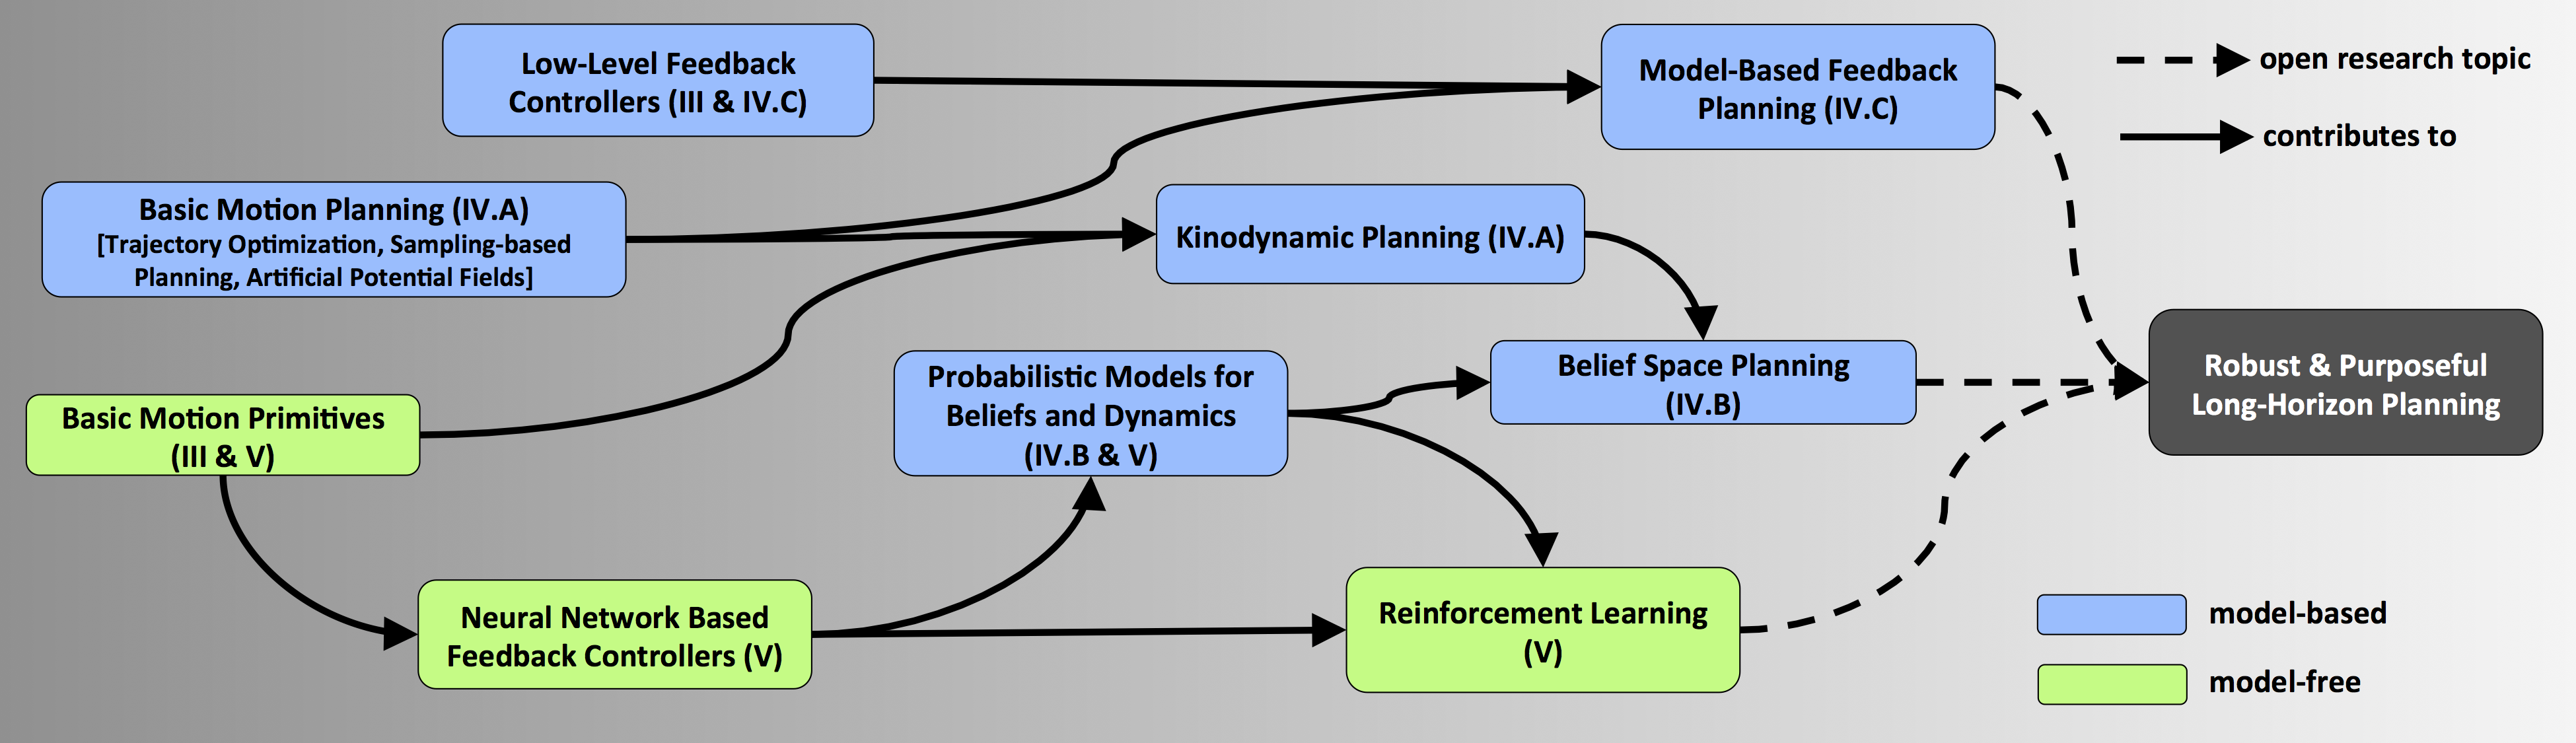
\includegraphics[width = \textwidth]{tex/img/review_overview_fig.png}
\vspace{-.2in}
\caption{Overview of research topics discussed. Numbers refer to
sections. An arrow indicates a topic that can contribute to the
development of another.  }
\vspace{-.2in}
\label{fig:overview}
\end{figure*}

\subsection{Methods for Controlling Soft Robots}

Soft materials can bend, twist, stretch, compress, buckle, wrinkle and
so on. Such motions may involve an infinite number of DoFs indicating
that the control if soft robots requires new approaches
\cite{Rus:2015aa, Trimmer:2014aa}. While some progress can 
be made with more traditional control approaches, such as Model
Predictive Control ({\tt MPC}), these efforts typically require
accurate models of the robot and environment, which can be difficult
to acquire given the complex physical properties of soft robots.
Thus, many efforts focus specifically on biomimetic
systems \cite{Kim:2013aa}, which aim to reproduce the control
behaviors of their biological counterparts and often provide a new
understanding of soft organisms~\cite{Lin:2011aa}.

%This is similar to developments in tensegrity
%structures \cite{skelton_tensegrity_2009}.

To better understand the challenges in controlling soft and tensegrity
based robots, new static, kinematic and dynamic models have been
developed to capture the ability of bending and flexing
\cite{Saunders:2011aa, skelton_tensegrity_2009}.  For many
years, a popular abstraction for soft robots has been that of
piece-wise constant curvature ({\tt PCC})
\cite{Webster:2010aa}, which does not
capture all aspects of real mechanisms. Recently some non-constant
curvature models have been proposed to better model soft mechanisms.
\cite{Renda:2014aa}.  The need for
expressive models has also led to the development of simulation tools
targeted to soft robots \cite{Germann:2013aa}. This is also an
important development in tensegrity
robotics \cite{Caluwaerts2013rsif}, in which open source physics based
simulation tools have recently become
available \cite{SunSpiralSoftware}.  Table~\ref{tbl:resources} gives
pointers to simulation tools and analytical models for tensegrity
structures.

There have been both model-based and model-free approaches for the
low-level control of soft robots \cite{Rigatos:2009aa}. On the
model-based side, a recent effort utilizes finite
elements \cite{Largilliere:2015aa}, while a recent data-driven,
model-free approaches utilizes graph-theory \cite{Vikas:2015aa}.
There is no consensus, however, yet regarding the appropriate
methodology for control, and especially planning, for soft robots
given their highly continuous, complex and intrinsically compliant
deformation \cite{Rus:2015aa}.  This has motivated efforts in
proposing behavior-based control architectures for soft robots that
may be applicable to tensegrities as well \cite{Armbrust:2015aa}.  A
critical challenge in achieving deliberative control and planning,
shared between tensegrity structures and soft robots, is the
difficulty of solving the inverse kinematics problem. There are
solutions in certain setups, such as for semi-soft
manipulators \cite{Neppalli:2009aa}.

% or under the {\tt PCC} assumption \cite{Marchese:2014aa}.

\subsection{Planning for Tensegrities}

Similar to soft robots, the very properties that make tensegrities
ideal for physical interaction with the environment, such as
compliance, and multi-path load distribution, present some significant
challenges to traditional planning approaches and lead to uncertainty
during motion execution.

For instance, compliance allows tensegrity robots to adapt their shape
to workspaces of unknown or uncertain geometry. But when a force is
applied, the robot can deform in a non-linear manner and will often
excite oscillatory behaviors \cite{SunSpiral2013Tensegrity-Base}.  The
results of contacts are therefore very hard to predict to the level of
accuracy required for traditional trajectory and route planning
techniques.  These issues have limited investigation of planning
algorithms and focused most existing efforts on controllers for the
generation of local gaits \cite{Paul2006a} and quasi-static
paths \cite{Porta:2015aa}. Yet, they have also inspired the
development of approaches that go beyond the traditional control
toolkit and allow adaptation to multiple different terrain
types~\cite{MirletzSoftRobotics,burms2015online}.  Similar
developments in soft robotics technologies are taking place, which
address the complications of self-loading and non-linear compliance
\cite{Rus:2015aa}.  Recently, planning methods have been introduced 
which begin to address these needs for soft
robots \cite{Bonilla:2015aa, Marchese:2016aa}.

To move this field forward for both tensegrity and soft robots, both
high-level approaches of model-based and model-free planning should be
investigated as highlighted in Fig.~\ref{fig:overview}.  Model-based
planning approaches should be able to reason over more complex
dynamical models of tensegrity systems and provide robust trajectories
over probabilistic state representations that capture the diversity of
possible executions given the inherent uncertainty. Another direction
is to study feedback-based motion planners that provide a robust
composition of controllers with performance guarantees. In the
model-free domain, methods should capture the dynamics of low-level
controllers and then plan over the resulting dynamics. The low-level
controllers should manage the details of environmental interaction
while successfully driving the system to the next waypoint.

%The rest of this paper will aim to review work in low-level control
%and planning for tensegrity robots and outline directions for further
%research in this domain given developments in the motion planning and
%robot learning fields.

%Many advances have been made in understanding how to control robots
%with these physical properties, but those very same desirable
%properties introduce significant challenges to long-range planning
%algorithms.  Specifically, the adaptability of the robots and their
%ability to behave in complex ways which are outside the scope of the
%control system makes long range planning difficult because there is
%much greater uncertainty about the evolution of the robot's state as
%it executes the desired plan.

\begin{table}[b]
\vspace{-.2in}
\centering
\begin{tabular}{r|r}
\textbf{resource} & \textbf{references} \\ \hline
\rowcolor[HTML]{BBDAFF} dynamics models   	& \cite{skelton_tensegrity_2009,hernandez2009reconfigurable,MiratsTur2009,sultan2002,Wroldsen2006A-Discussion-on}\\
kinematics \& statics
& \cite{C.R.1978,6907473,skelton_tensegrity_2009, 2003Tensegrity:-Str,Guest2010,Juan2008,pellegrino2014deployable}           \\
\rowcolor[HTML]{BBDAFF} simulation        	& \cite{SunSpiralSoftware,MirletzSoftRobotics,skelton_tensegrity_2009,Caluwaerts2013rsif,Rovira2009Control-and-Sim} \\
hardware design
                        & \cite{Bliss2013Central-Pattern,bohm2013vibration,Fest2004,Shibata2009,Caluwaerts2013rsif,miratstur2011athree-dof,kimrobust,Khazanov:2014aa,ChanMarch2004} \\
                        & \cite{Koizumi2012b,Paul2006a,Rieffel2009,Mirletz2015,sabelhaus2015system,bruce2014design,veuve2015deployment} \\
\rowcolor[HTML]{BBDAFF} state estimation        & \cite{Caluwaerts:2015aa} 
\end{tabular}
\caption{\vspace{-.05in}Resources for tensegrity control.}
%\vspace{-.4in}
\label{tbl:resources}
\end{table}

%dos2015design,fest2003adjustable


\section{Low-level Control for Tensegrity Robots}
\label{sec:control}
Early tensegrity research was mostly focused on modeling the statics
~\cite{2003Tensegrity:-Str, Juan2008, Arsenault:2008bh} and dynamics
of a structure, so as to provide effective equations of motion
~\cite{Kanchanasaratool2002Motion-Control-, De-Oliveira:2006ys,
skelton_tensegrity_2009}.  In specific cases, such as state
estimation, modeling tensegrities as constrained mass-spring nets
allows for highly efficient and sufficiently accurate
implementations~\cite{Caluwaerts:2015aa}.  The mass-spring approach
has also proven valuable in more theoretical studies of morphological
computation~\cite{Hauser}. Nevertheless, there is a trade off between
computational efficiency and high dynamic model fidelity during
environment interaction modeling.  Table~\ref{tbl:resources}
summarizes many of these contributions that can impact tensegrity
control.

%But the dynamics of tensegrities is an active research area being
%approached by a variety of viewpoints~\cite{skelton_tensegrity_2009}.


Many of the tensegrity hardware robots are tendon-driven or use
pneumatic actuators, which are typically a burden to accurately model
analytically. A learned model might increase the computational
efficiency when trying to represent real-world hardware in changing
environments.  Section~\ref{sec:learning} discusses the option of
using learned models as a proxy to simulation or involved analytical
models.

%Given models of tensegrity structures, many interesting problems
%regarding tensegrity structures correspond to their
%control \cite{Tur:2009fu}.

Given a dynamic model, it is possible to control a tensegrity
structure along static equilibrium
manifolds~\cite{Skelton1997Controllable-Te}.  Alternatively, feedback
linearization control laws~\cite{Aldrich2003Control-Synthes} or
Lyapunov-based controllers for 3D dynamic
models~\cite{Wroldsen2006A-Discussion-on} have also been
developed. Frequently, these approaches do not account for
self-collisions or environmental contact dynamics, limiting their
real-world applicability.  Planning processes for a real-world
tensegrity structure need to utilize modeling and simulation tools
that take collisions into account.

%This is an important component of simulation tools, which can help to
%study controlled actuation, as these collisions generate the forces
%to propel the system~\cite{Rovira2009Control-and-Sim,
%Wittmeier2011CALIPER:-A-univ}.

Many efforts focus on generating efficient gaits, defined as rhythmic
motions, which lead to nonzero movement of the center of
mass~\cite{McIsaac:2003kl}.  Given the high-dimensional nature of the
search space, genetic algorithms are frequently applied to achieve
forward locomotion gaits~\cite{Paul2006a}. Evolutionary algorithms
have been used for generating irregular locomotion and civil
engineering structures~\cite{Rieffel2009Automated-Disco,
veuve2015deployment}. Recently, evolutionary methods have been
proposed that utilize a multi-agent learning
approach~\cite{Iscen2013Controlling-Ten}.  Other biologically-inspired
approaches based on Central Pattern Generators (CPGs) have also
been applied to tensegrity-based
systems~\cite{Bliss2013Central-Pattern, MirletzSoftRobotics,
Caluwaerts2013rsif}. 
A recent overview of low-level tensegrity
control approaches is available in the related literature~\cite[Table
2]{Caluwaerts2013rsif}. 
In this work, we train Artificial Neural Networks (ANNs) as open loop controllers for locomotion.
Then use the ANNs to train closed looped CPGs to get controllable locomotion.
Section~\ref{sec:NN_and_CPG_overview} gives a basic overview of ANNs and CPGs.

% \begin{figure*}[t]
% \includegraphics[width=0.235\textwidth]{figures/_0_1_extended.jpg}
% \hspace{0.05in}
% \includegraphics[width=0.235\textwidth]{figures/_0_3_extended.jpg}
% \hspace{0.05in}
% \includegraphics[width=0.235\textwidth]{figures/_0_5_extended.jpg}
% \hspace{0.05in}
% \includegraphics[width=0.235\textwidth]{figures/_0_7_extended.jpg}
% \vspace{-.25in}
% \caption{\footnotesize Resulting trajectory for a physically simulated
%   tensegrity robot \cite{SunSpiralSoftware} using an asymptotically, 
%   near-optimal kinodynamic planner
%   \cite{Li2015Sparse-Methods-}.}
%  \vspace{-.2in}
% \label{fig:tens_example}
% \end{figure*}

%such as an experimental robotic
%swimmer \cite{Bliss2013Central-Pattern}, spine-like
%tensegrities~\cite{Tietz2013Tetraspine:-Rob} and the tensegrity
%icosahedron~\cite{Caluwaerts2013rsif}.  

%This line of work tries to take advantage of the fact that forces in tensegrity structures tend to propagate in a distributed way.

%What should the future hold for low-level tensegrity control methods?

The availability of simulation tools has offered researchers the
possibility to develop a wide range of controllers.  Nevertheless,
additional hardware validation results are needed to better support
the claims regarding the efficacy of the developed
solutions~\cite{Mirletz2015, Caluwaerts2013rsif}.  It is crucial to
determine the feasibility of each method in terms of sensing and state
estimation, their aptitude for distributed implementations and the
minimum number of actuators required.

Furthermore, hardware experiments have not typically utilized
fundamental analytical control approaches (e.g.~\cite{sultan2002}),
since they frequently depend on accurate state information, which is
non-trivial to acquire.  Nevertheless, there has been recent progress
on actuation, sensing, and state-estimation methods that are robust to
noisy sensors and environments.  Thus, it may be time to revisit some
of the earlier analytical control techniques. This will allow a
thorough comparison with more modern methods that have reduced sensing
and actuation requirements in simulation and hardware.

%This will serve as a springboard for the
%development of useful local maneuvers for tensegrity robots that can
%be used for long-term mobility purposes in the context of realistic
%terrains and for three-dimensional, large, irregular tensegrity
%structures.

%\komment{Ken: Do we need the above paragraph? Kostas: I personally like it
%because it takes a stance. It is a reasonable recommendation.}

%Low-level controllers can provide primitives that can be used as
%building blocks for global path planning approaches.  For this to be
%plausible, a common parametrization for low-level controllers is
%needed and a method to predict the probability of success or the
%region of attraction of a controller when a low-level controller is
%activated to transition between desired states

%\komment{Ken: I don't like the above sentence, but we need its message in
%the paper Kostas: Since it is going to appear later, perhaps we do not
%need to say it here.}


\section{Neural Net and Central Pattern Generators for Tensegrity Robots}
\label{sec:NN_and_CPG_overview}

\subsection{Artificial Neural Networks}
Artificial Neural Networks (ANNs) are a theoretical group of mathematical models loosely based on neural networks found in biology that can estimate usually unknown functions which map multiple inputs to a set of outputs.
An ANN is comprised of a large set of simple functions grouped into different layers that define a mapping function \(f:X \to Y\) where \(X\) is the input set and \(Y\) is the output set.
In practice, layers are grouped into three main layers defined as 1) the Input layer, 2) the Hidden layer, and 3) the Output layer.
The Input and Output layers transfer data to and from the Hidden layer, respectively.
The Hidden layer can be comprised of one ore more sub-layers and is where the input data is converted to the output data.
Each sub-layer of the Hidden layer is comprised of a defined number of simple functions \(H_{i}\) for \(i \in n\), where \(n\) is total number of functions in a sub-layer.
Changing how each function \(h \in H\) is connected to other functions, by the use of weights, allows for the ANN to map its inputs to a desired output~\cite{lippmann1987introduction}~\textcolor{red}{Probably should reference more}. For our application, machine learning is used to estimate the connection weights through the use of a cost function.
The cost function is an equation which measures how close to a user defined goal an iteration during the learning process was able to achieve.

\subsection{Central Pattern Generators}
\label{sec:CPG_overview}
Central Pattern Generators, or CPGs, are a set of two or more rhythmic processes connected such that each output interacts with the other process(es) to sequentially decrease and increase each process' output.
The benefit of such a network for rhythmic generators is that, once started, the network will have a series of rhythmic outputs that are phase offset from each other with no need for any external sensory input.
Discovered over a hundred years ago~\cite{brown1911intrinsic} and formally observed and named in the early 1960's~\cite{wilson1961central}, CPGs have linked to many rhythmic biological systems e.g. vertebrate walking~\cite{brown1911intrinsic,grillner2006biological} and involuntary movements~\cite{janczewski2006distinct,robertson1981oscillatory}.


% Because  of  the  limited  research  into  actuated  tensegrity
% robotics,   many   design   aspects   have   yet   to   be   carefully
% studied. To date, the majority of constructed tensegrity robots
% have  been  simple  prototypes  using  servo  motors,  limited
% sensing,  and  are  often  tethered  for  power  and  control  [5].
% Others have had fewer limbs than the SUPER ball, or have
% been  secured  to  the  ground  as  opposed  to  free-standing
% [6][7]. Some related approaches utilize tensegrity as part of a
% larger, more complicated system, but not as the primary loco-
% motion method [8]. Others have created designs that do not
% use direct cable actuation, as in the SUPER ball, but instead
% have  more  limited  forms  of  locomotion  through  vibration
% [9][10]. Finally, the most similar designs to the SUPER ball
% have not been engineered to specific design requirements nor
% have  the  advanced  sensing  framework  needed  for  controls
% testing [11]
%
% The  high  strength-to-weight  ratio  of  tensegrity  structures
% is very attractive due to the impact of mass on mission launch
% costs.  Large  tensegrity  structures  have  been  shown  to  be
% deployable from small compact configurations which enable
% them to fit into space constrained launch fairings. While the
% above qualities have inspired studies of deployable antennae
% and  other  large  space  structures  [12],  it  is  in  the  realm
% of  planetary  exploration  that  we  see  the  most  significant
% role  for  many  of  the  unique  force  distribution  qualities  of
% tensegrity  robots.  A  recent  NIAC  project  [13]  specifically
% studies  landing  and  surface  mobility  of  tensegrities,  ex-
% ploiting  the  controllable  compliance  and  force  distribution
% properties which make for reliable and robust environmental
% interactions.
% The   main   goal   is   to   develop   tensegrity   probes   with
% an  actively  controllable  tensile  network  to  enable  compact
% stowage  for  launch,  followed  by  deployment  in  preparation
% for  landing.  Due  to  their  natural  compliance  and  structural
% force  distribution  properties,  tensegrity  probes  can  safely
% absorb significant impact forces, enabling high speed Entry,
% Descent, and Landing (EDL) scenarios where the probe itself
% acts  much  like  an  airbag.  However,  unlike  an  airbag  which
% must  be  discarded  after  a  single  use,  the  tensegrity  probe
% can  actively  control  its  shape  to  provide  compliant  rolling
% mobility  while  still  maintaining  the  ability  to  safely  absorb
% impact  shocks  that  might  occur  during  exploration.  This
% combination  of  functions  from  a  single  structure  enables
% compact and lightweight planetary exploration missions with
% the capabilities of traditional wheeled rovers, but with a mass
% and cost similar or less than a stationary probe.
%
% Therefore, a large fraction of the overall weight (as mea-
% sured  at  atmospheric  entry)  of  a  tensegrity  mission  can  be
% used  for  the  scientific  payload  due  to  the  dual  use  of  the
% structure  as  a  lander  and  a  rover.  This  allows  for  cheaper
% missions  and  enable  new  forms  of  surface  exploration  that
% utilize the natural tolerance to impacts of tensegrities [14].
%
% Buckminster Fuller [1] and the artist Kenneth Snelson [2]
% initially  explored  tensegrity  structures  in  the  1960s.  Until
% the  mid-1990s  the  majority  of  tensegrity  related  research
% was  concerned  with  form-finding  [15]  and  design  analysis
% of  static  structure  [16][17].  More  recently,  active  control
% efforts  for  tensegrities  began  to  emerge  [18],  as  well  as
% descriptions  of  the  dynamics  of  tensegrity  structures  taking
% the connectivity pattern into account [17].
% The tensegrity principle allows for compliance and multi-
% path load distribution, which is ideal for physical interaction
% with  the  environment.  However,  these  aspects  also  present
% significant  challenges  to  traditional  control  approaches.  A
% recent  review  [19]  shows  that  there  are  still  many  open
% problems in actively controlling tensegrities, especially when
% interacting  with  an  environment  during  locomotion  or  ma-
% nipulation  tasks.  Though  work  has  been  done  to  control  a
% tensegrity  to  change  into  a  specified  shape  [20],  practical
% determination  of  the  desired  shape  itself  is  an  ongoing
% challenge.  Recently,  locomotion  of  icosahedral  tensegrity
% robots  through  body  deformation  was  demonstrated  [21].
% Other work has addressed collision between rigid tensegrity
% elements during control generation [22][23].
% The  approach  taken  by  the  NASA  Dynamic  Tensegrity
% Robotics  Lab  builds  on  this  by  developing  body  defor-
% mation  control  algorithms  based  on  central  pattern  gen-
% erators  [24][25],  distributed  learning,  reservoir  computing,
% and  genetic  algorithms  [26],  instead  of  traditional  linear
% and  nonlinear  systems  approaches.  To  date,  our  approach
% has  shown  promising  results  at  productively  harnessing  the
% potential  of  complex,  compliant,  and  nonlinear  tensegrity
% structures.

% \section{Motivation an Goal}
